%%
%%  Annexes
%%
%%  Note: Ne pas modifier la ligne ci-dessous. / Do not modify the following line.
\ifthenelse{\equal{\Langue}{english}}{
	\addcontentsline{toc}{compteur}{APPENDICES}
}{
	\addcontentsline{toc}{compteur}{ANNEXES}
}
%%
%%
%%  Toutes les annexes doivent être inclues dans ce document
%%  les unes à la suite des autres.
%%  All annexes must be included in this document one after the other.
\Annexe{Matériaux élastomères alternatifs}

En plus des essais présentés concernant le PEI-siloxane, des élastomères SIS et SEBS ont été initialement évalués pour ce projet. 
Ces matériaux ont été sélectionnés par Adrien Métafiot durant une partie de son doctorat. 

\section{Matériaux}

Les deux élastomères initialement évalués étaient : 
\begin{inparaenum}[]
	\item un copolymères triblocs polystyrène-b-polyisoprène-b-polystyrène (SIS) possédant une fraction molaire de styrène de 22\% (Sigma-Aldrich \#432415) et 
	\item un copolymère triblocs linéaire polystyrène-b-poly(éthylène-butylène)-b-polystyrène (SEBS) produit par Kraton\textregistered \ sous le numéro de désignation A1536 H. 
\end{inparaenum}
Les copolymères triblocs possèdent une structure générale où un segment est inséré au milieu de deux segments possédant une composition différente au segment central (Fig. \ref{fig:polymere_tri_bloc}). 

\section{Caractérisation de la stabilité thermique des élastomères}

Des analyses thermogravimétriques (TGA) de l'élastomère ont été réalisées avec un appareil TA Instruments Q50. 
Deux types d'analyses ont été réalisés. 
Dans un premier temps, tel que présenté dans la norme ASTM E2550 - 17, les échantillons ont été soumis à une rampe de \SI[locale=FR]{10}{\celsius\per\minute} jusqu'à une température de \SI[locale=FR]{575}{\celsius} sous une atmosphère régulière et sous une atmosphère d'azote. 
Par la suite, certains échantillons ont été également testés en condition isotherme autant avec une atmosphère d'air qu'avec une atmosphère d'azote pour évaluer la stabilité thermique dans le temps de l'élastomère. 
Ce second type d'analyse ne fait pas l'objet d'une norme standardisée de l'ASTM. 

\section{Stabilité thermique des élastomères}

Des mesures de thermogravimétrie ont été réalisées par Adrien Métafiot à McGill durant son doctorat afin d'observer le comportement thermique des élastomères SIS et SEBS. 
Dans un premier temps, un élastomère copolymère SIS commercial a été évalué. 
Les essais de caractérisation thermique (Fig. \ref{fig:TGA_SIS}) ont rapidement indiqué que ce matériau ne rencontrerait pas les requis techniques. 
Même après un traitement d'hydrogénation ses performances mécaniques restaient insuffisantes. 
À son état vierge, le SIS commercial s'est dégradé rapidement au-dessus d'une température de \SI[locale=FR]{320}{\celsius} (Fig. \ref{fig:TGA_SIS_vierge}) tandis qu'après le traitement d'hydrogénation, l'élastomère a conservé 99,5\% de sa masse jusqu'à une température de \SI[locale=FR]{325}{\celsius} (Fig. \ref{fig:TGA_SYS_hydrogenated}) et présentait ensuite un début de dégradation plus progressif.  
Ce matériau a été rejeté avant d'atteindre le stade des essais de soudage. 

\begin{figure}[h]
	\centering
	\subfigure[]
	{\label{fig:TGA_SIS_vierge} 								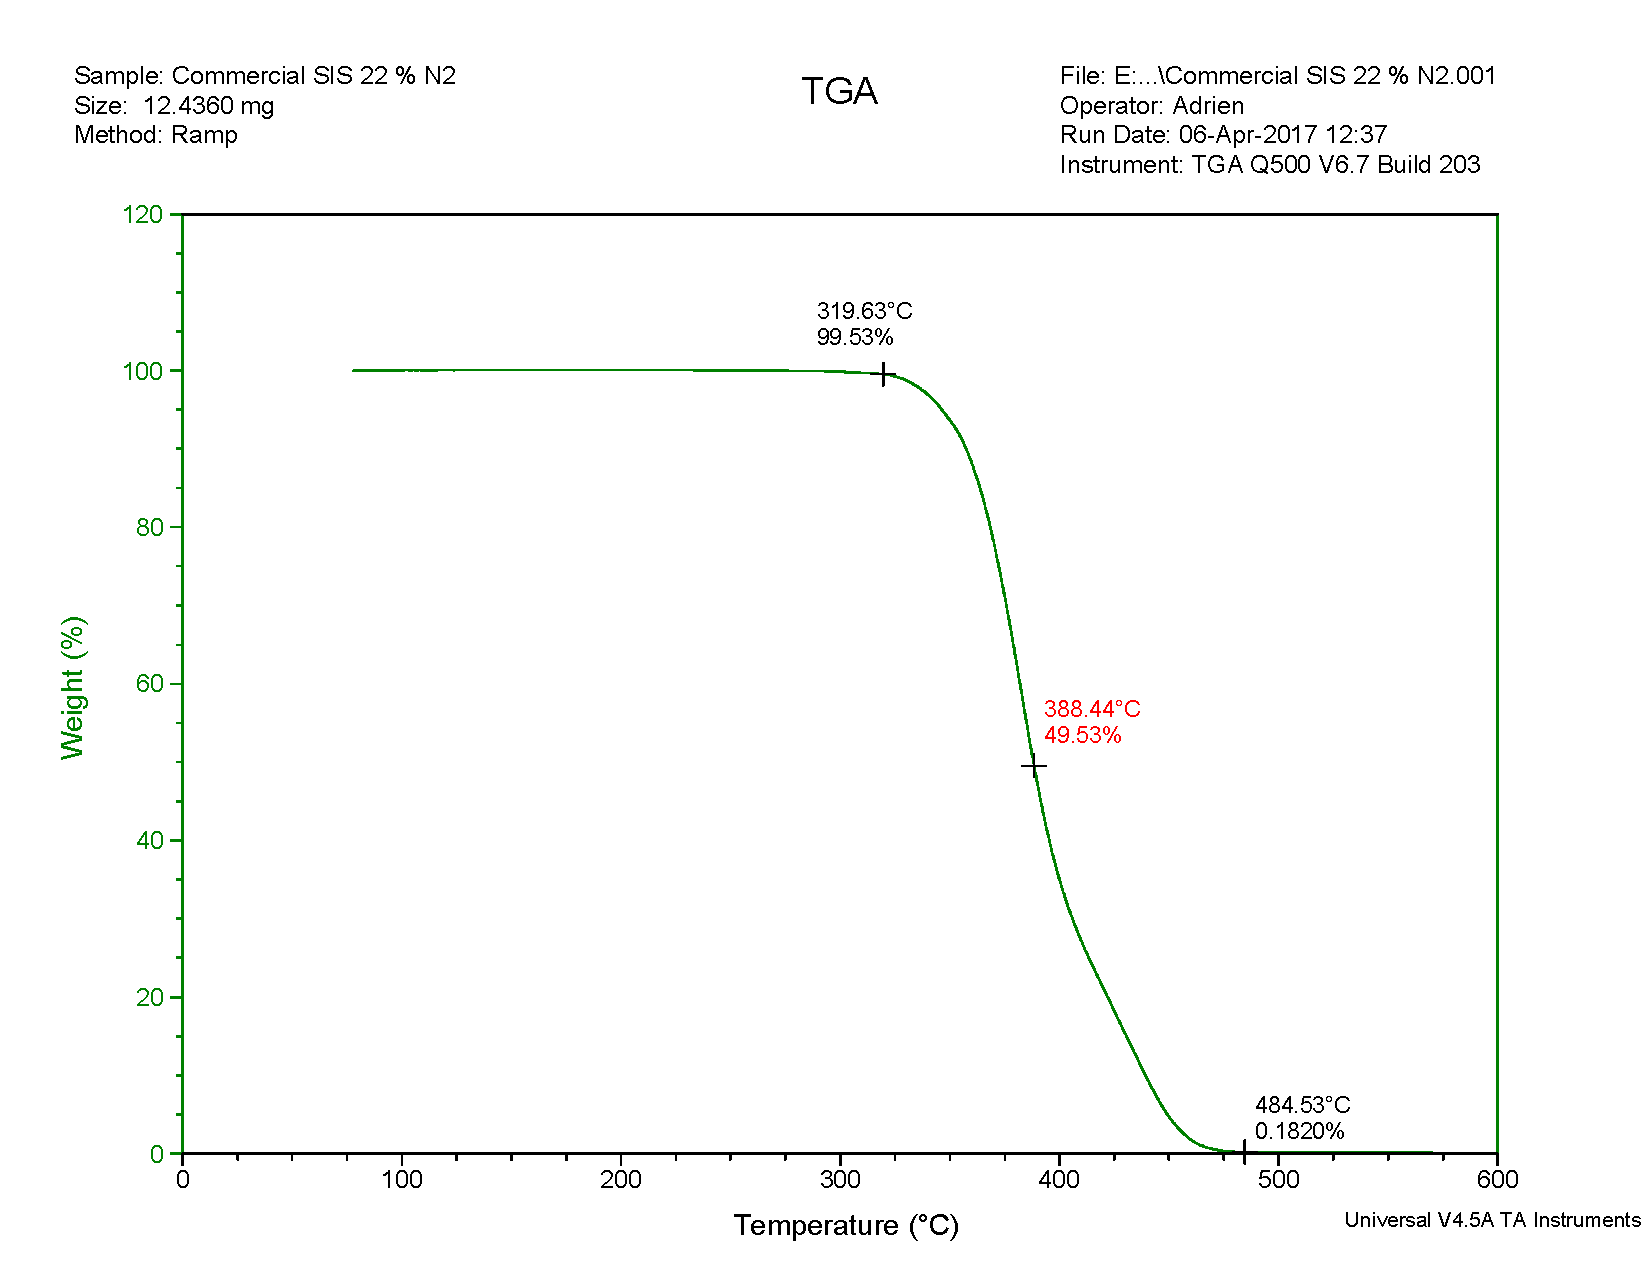
\includegraphics[width=0.75\textwidth]{TGA_Commercial_SIS_22p100_N2.pdf}
	}\\
	\subfigure[]
	{\label{fig:TGA_SYS_hydrogenated}
		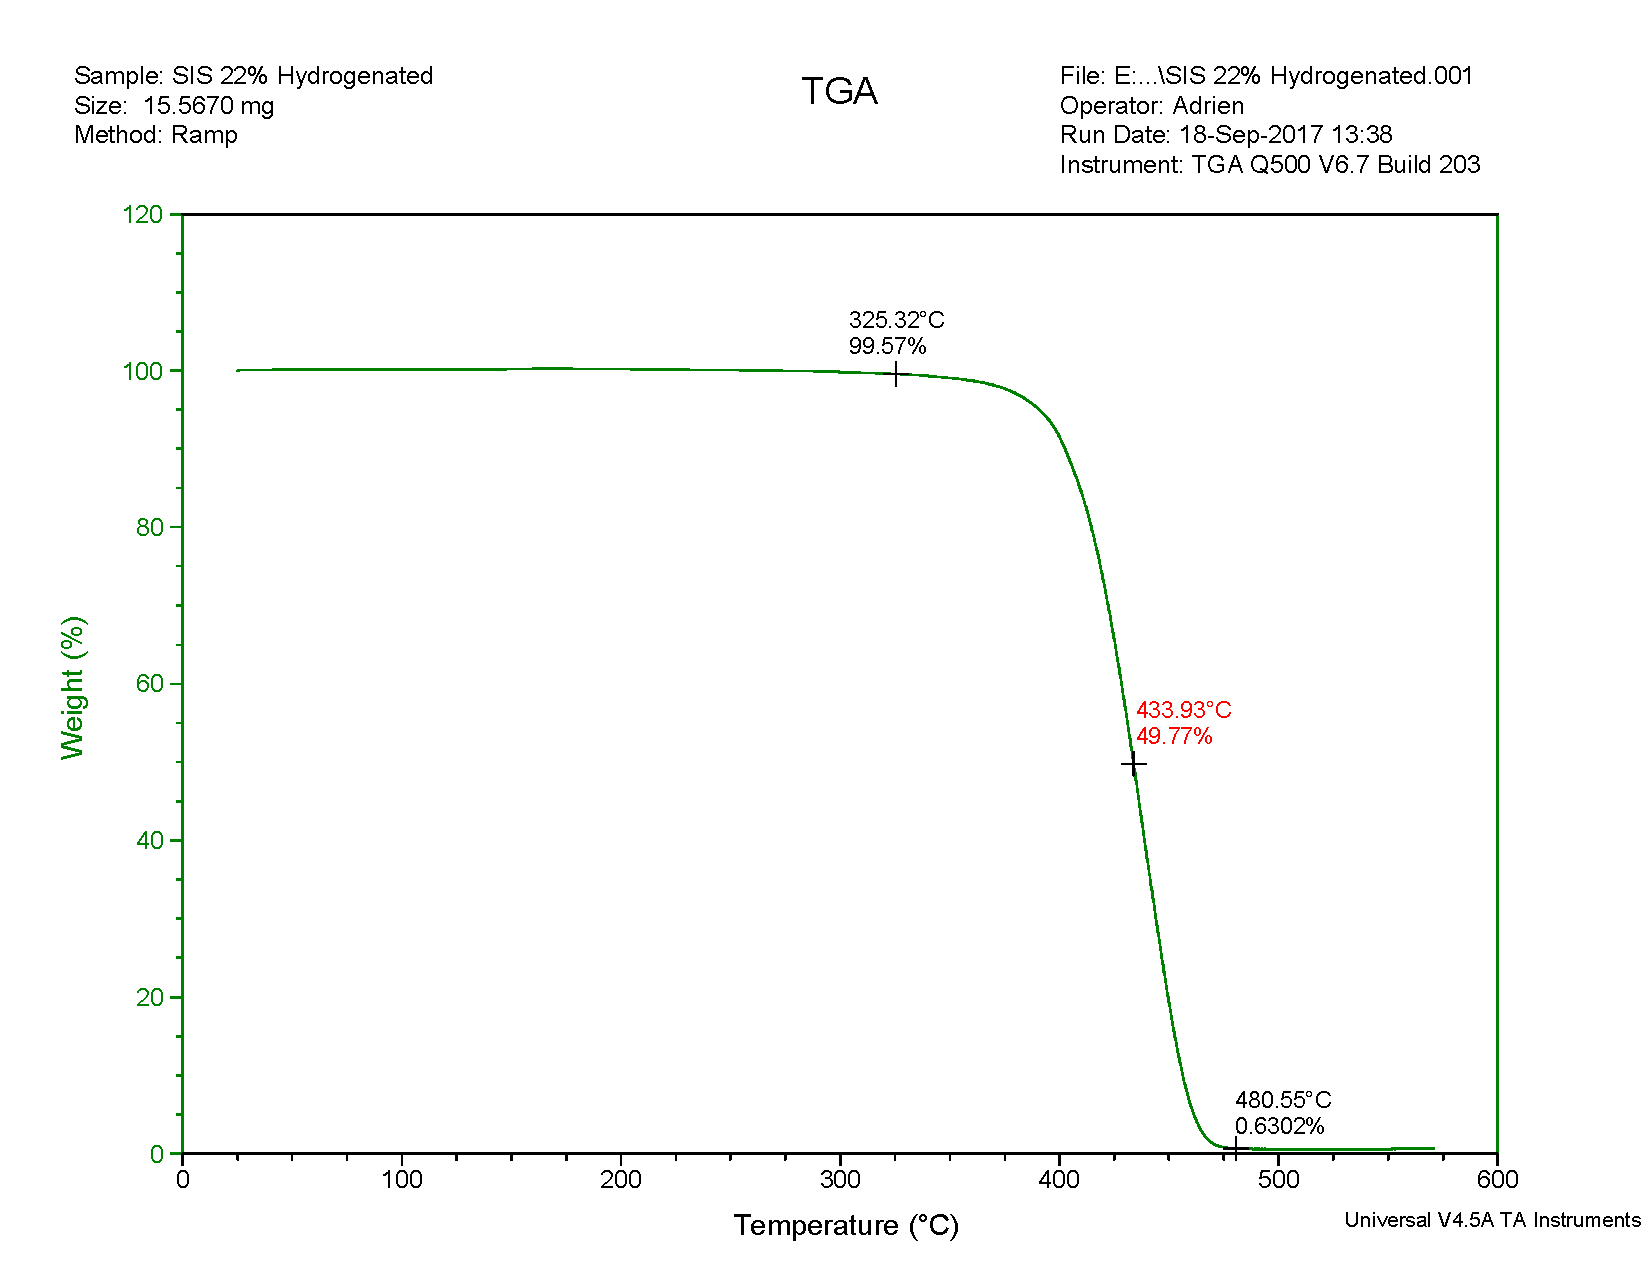
\includegraphics[width=0.75\textwidth]{TGA_Commercial_SIS_22p100_Hydrogenated_N2.pdf}
	}
	\caption{Résultats en TGA sous une atmosphère d'azote pour l'élastomère SIS commercial avec 22\% de styrène, a) SIS vierge, b) SIS ayant subi un traitement d'hydrogénation}
	\label{fig:TGA_SIS}
\end{figure}

En second lieu, le copolymère linéaire tribloc SEBS a été évalué. 
Les essais sous atmosphère standard (Fig. \ref{fig:TGA_rampe_SEBS_air}) ont démontré une dégradation rapide au-dessus de \SI[locale=FR]{270}{\celsius}. 
Cependant, puisque l'élastomère du joint n'est pas exposé directement à l'atmosphère durant le soudage, des essais sous atmosphère d'azote ont également été réalisés. 
Dans ces conditions, le SEBS a démontré une meilleure stabilité thermique que le SIS (Fig. \ref{fig:TGA_rampe_SEBS_N2}) avec des signes de dégradation observables seulement au-dessus de \SI[locale=FR]{340}{\celsius}. 

\begin{figure}[h]
	\centering
	\subfigure[]
	{\label{fig:TGA_rampe_SEBS_air} 								
		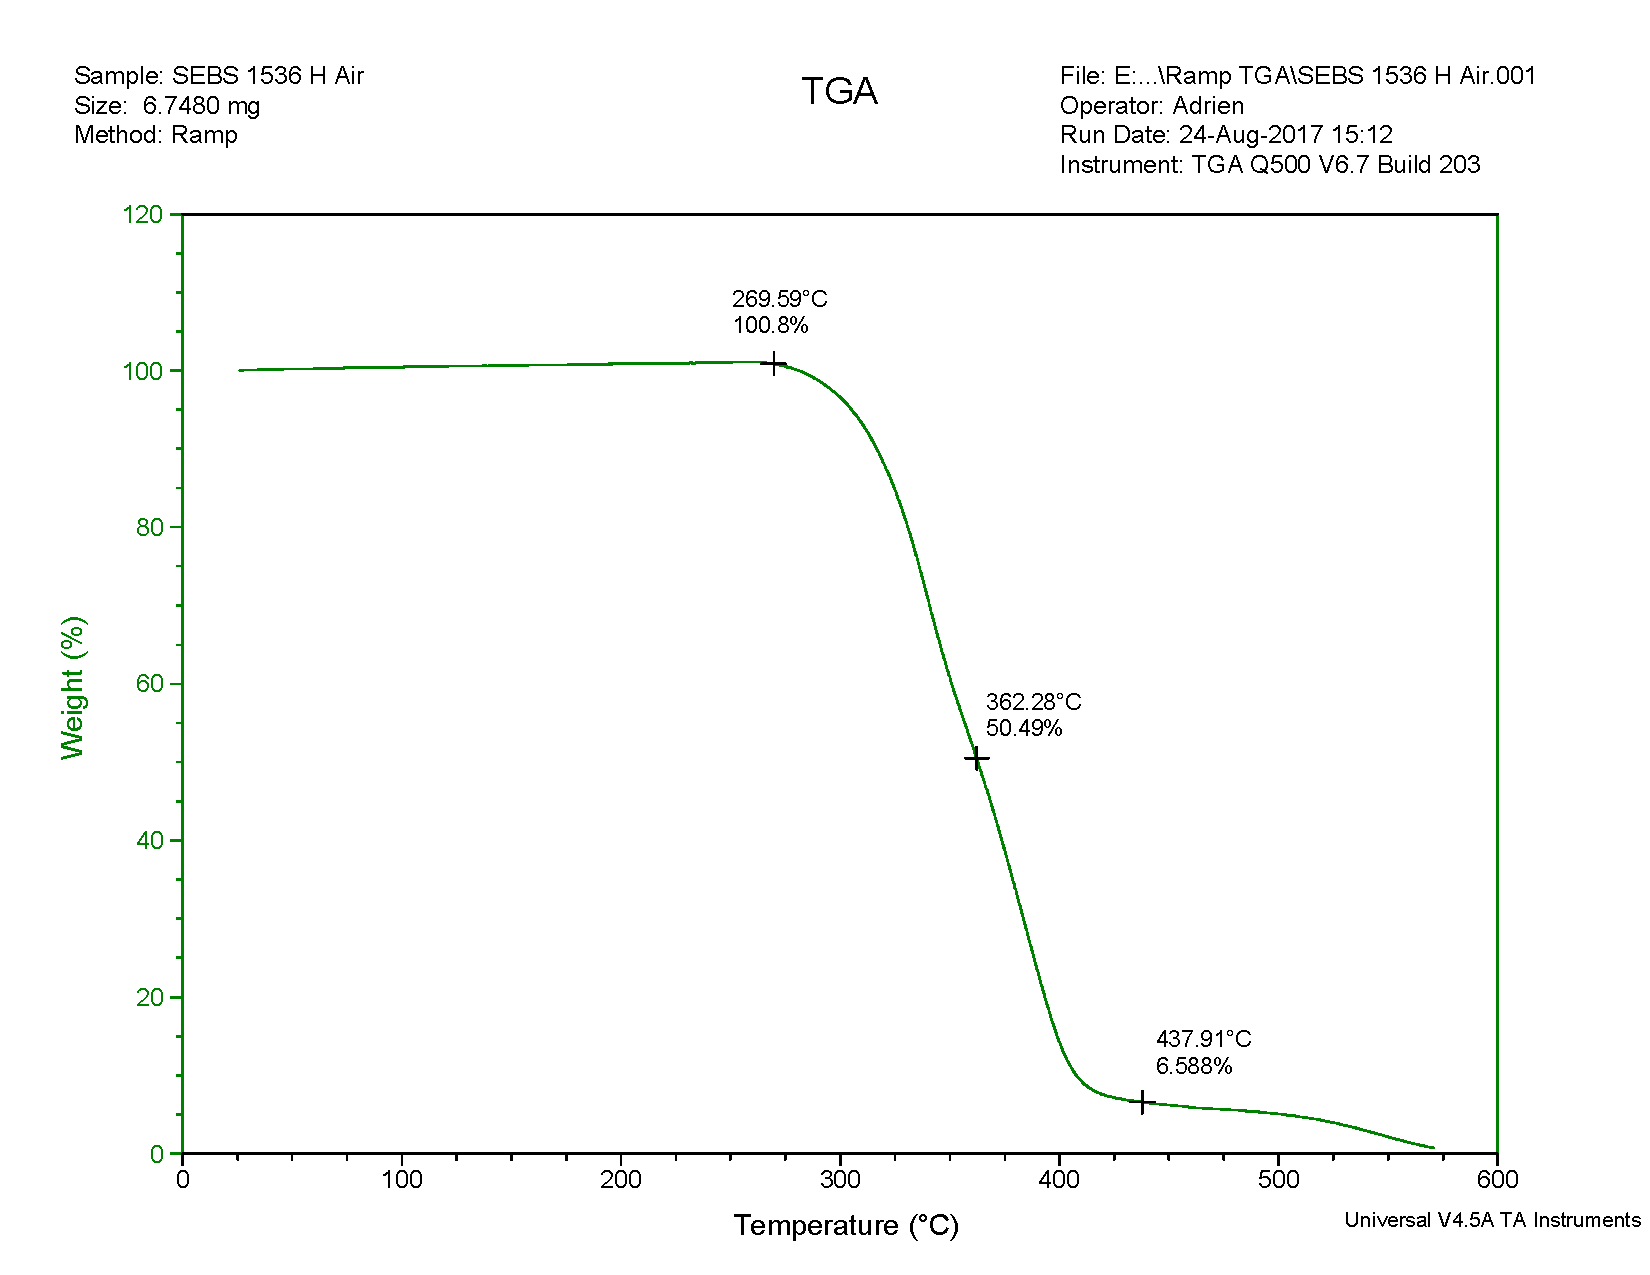
\includegraphics[width=0.75\textwidth]{TGA_SEBS_1536H_Air.pdf}
	}\\
	\subfigure[]
	{\label{fig:TGA_rampe_SEBS_N2}
		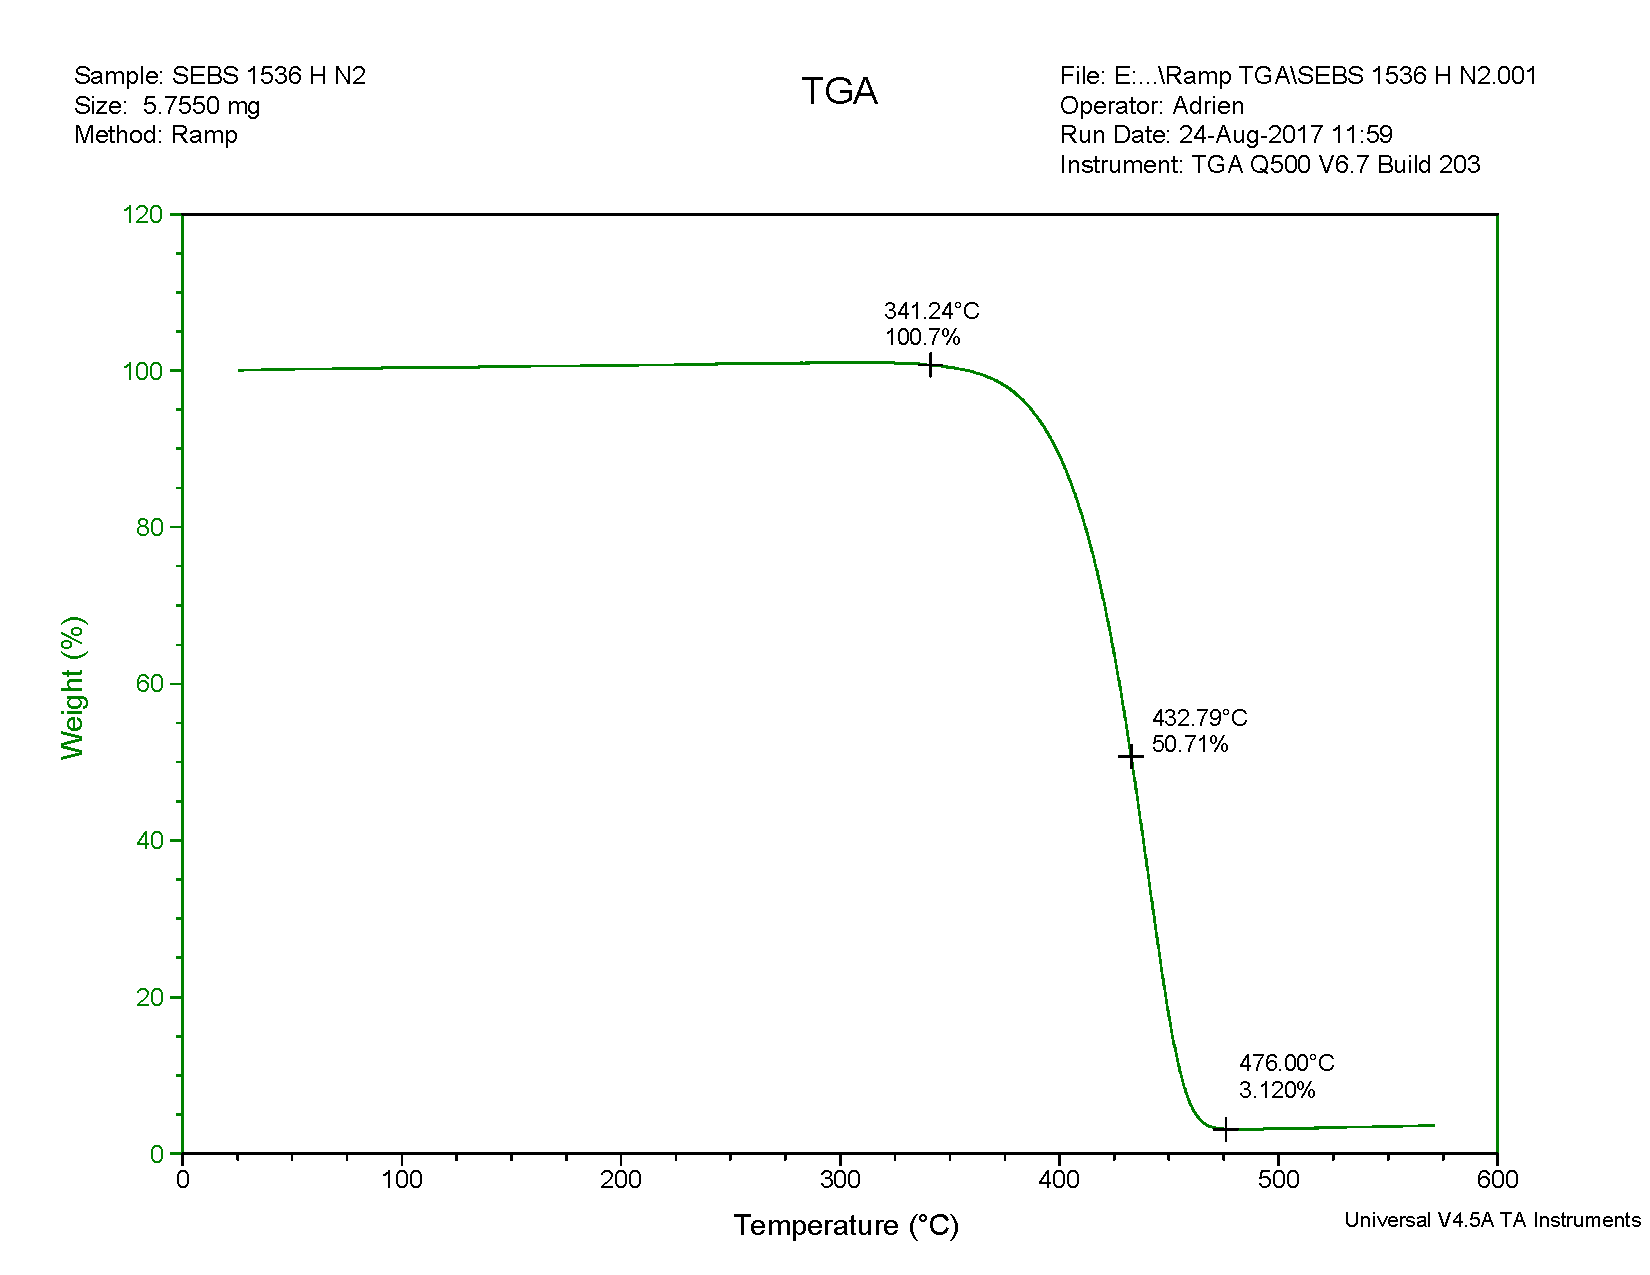
\includegraphics[width=0.75\textwidth]{TGA_SEBS_1536H_N2.pdf}
	}
	\caption{Résultats en TGA l'élastomère SEBS dans une atmosphère a) d'air, b) d'azote}
	\label{fig:TGA_rampe_SEBS}
\end{figure}

Il a été décidé de pousser plus loin l'analyse thermique de cet élastomère avec des essais de TGA isotherme. 
Les essais en isotherme sont beaucoup plus demandants que les essais standards avec une rampe de température. 
Cette méthode de test permet de valider hors de tout doute la stabilité thermique d'un polymère. 
Lorsque le test est réalisé avec une atmosphère standard (Fig. \ref{fig:TGA_iso_SEBS_air}), on observe une bonne stabilité thermique à \SI[locale=FR]{200}{\celsius} (Fig. \ref{fig:TGA_iso_SEBS_air_200}), mais on observe une dégradation thermique lente quand on répète l'essai à \SI[locale=FR]{230}{\celsius} (Fig. \ref{fig:TGA_iso_SEBS_air_230}). 
Quand cet essai est plutôt réalisé sous une atmosphère d'azote (Fig. \ref{fig:TGA_iso_SEBS_N2}), on observe des températures de dégradation légèrement plus élevées. 
Le SEBS est stable lorsqu'il est soumis à une température de \SI[locale=FR]{275}{\celsius} (Fig. \ref{fig:TGA_iso_SEBS_N2_275}), mais il commence à se dégrader lorsqu'il est soumis à une température de \SI[locale=FR]{290}{\celsius} (Fig. \ref{fig:TGA_iso_SEBS_N2_290}). 

\begin{figure}[h]
	\centering
	\subfigure[]
	{\label{fig:TGA_iso_SEBS_air_200} 								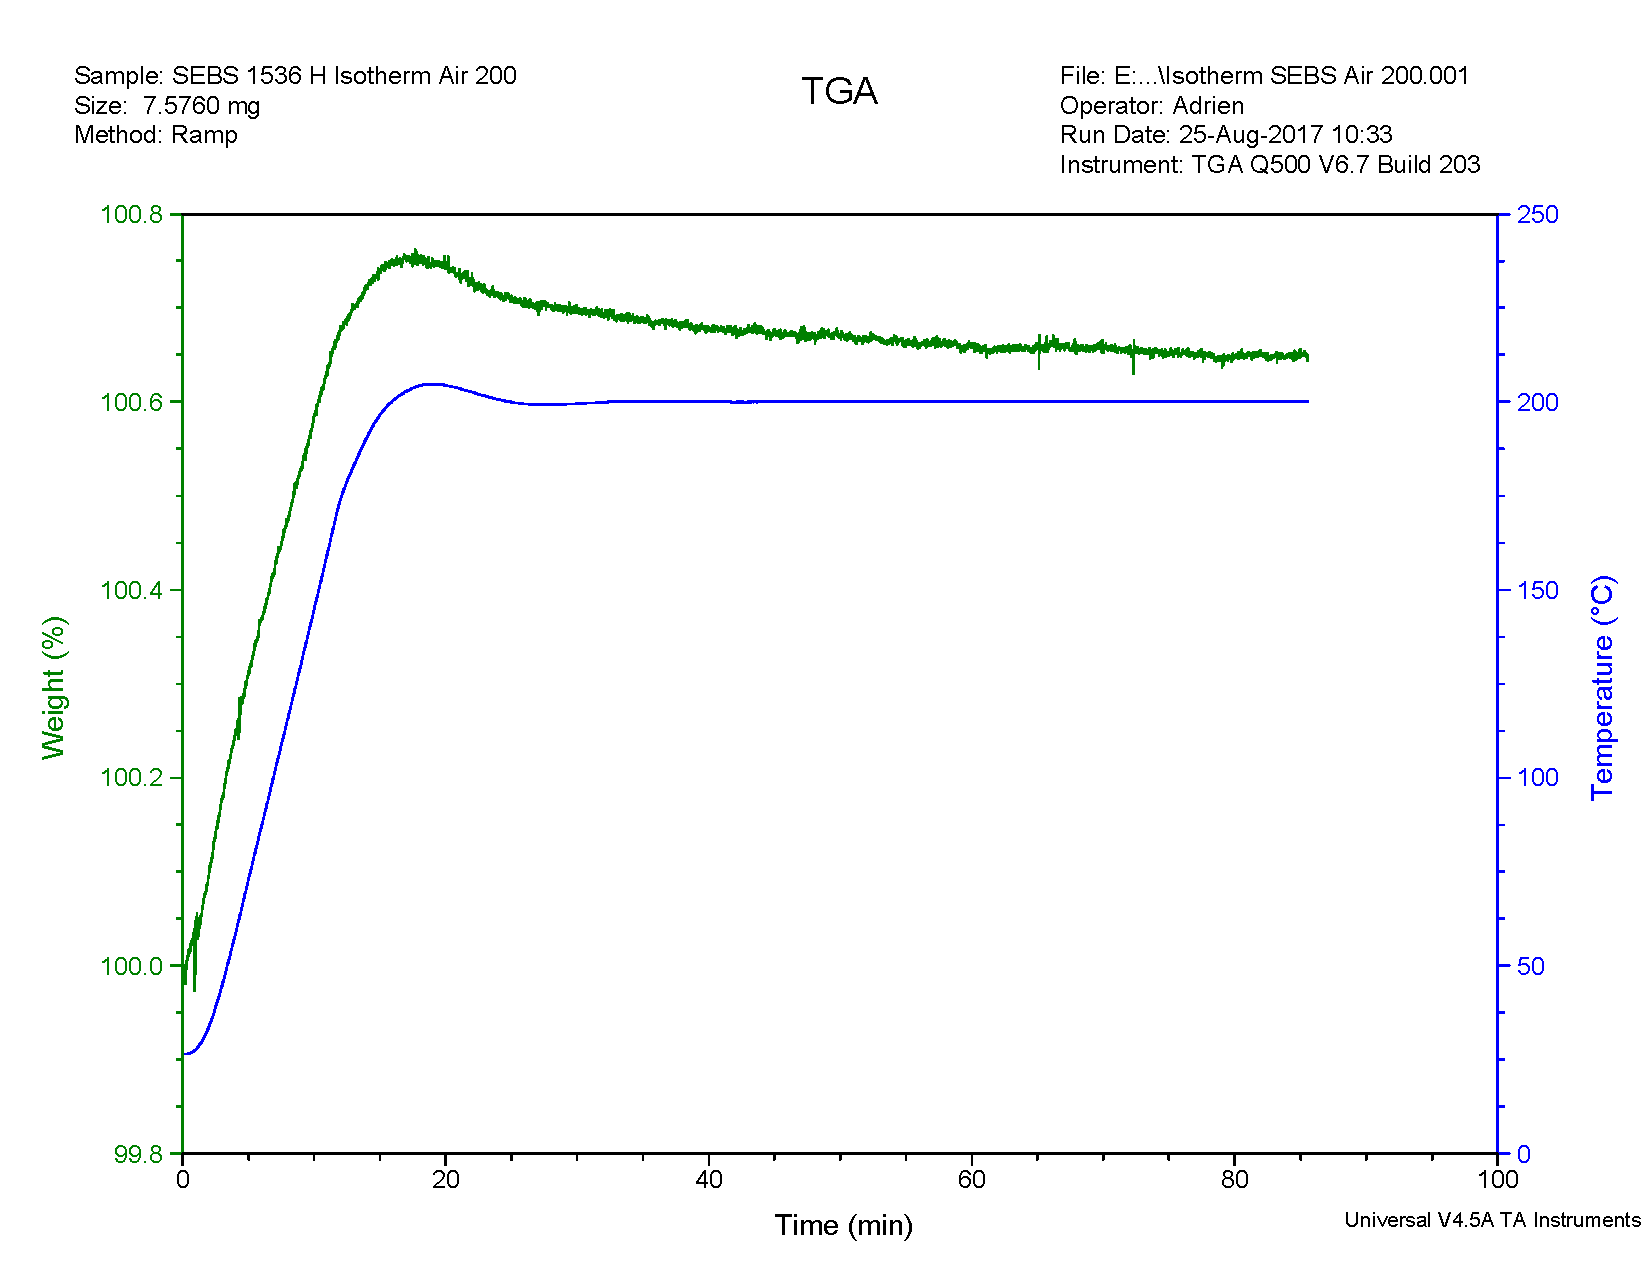
\includegraphics[width=0.75\textwidth]{TGA_SEBS_1536H_Air_Isotherm_200.pdf}
	}\\
	\subfigure[]
	{\label{fig:TGA_iso_SEBS_air_230}
		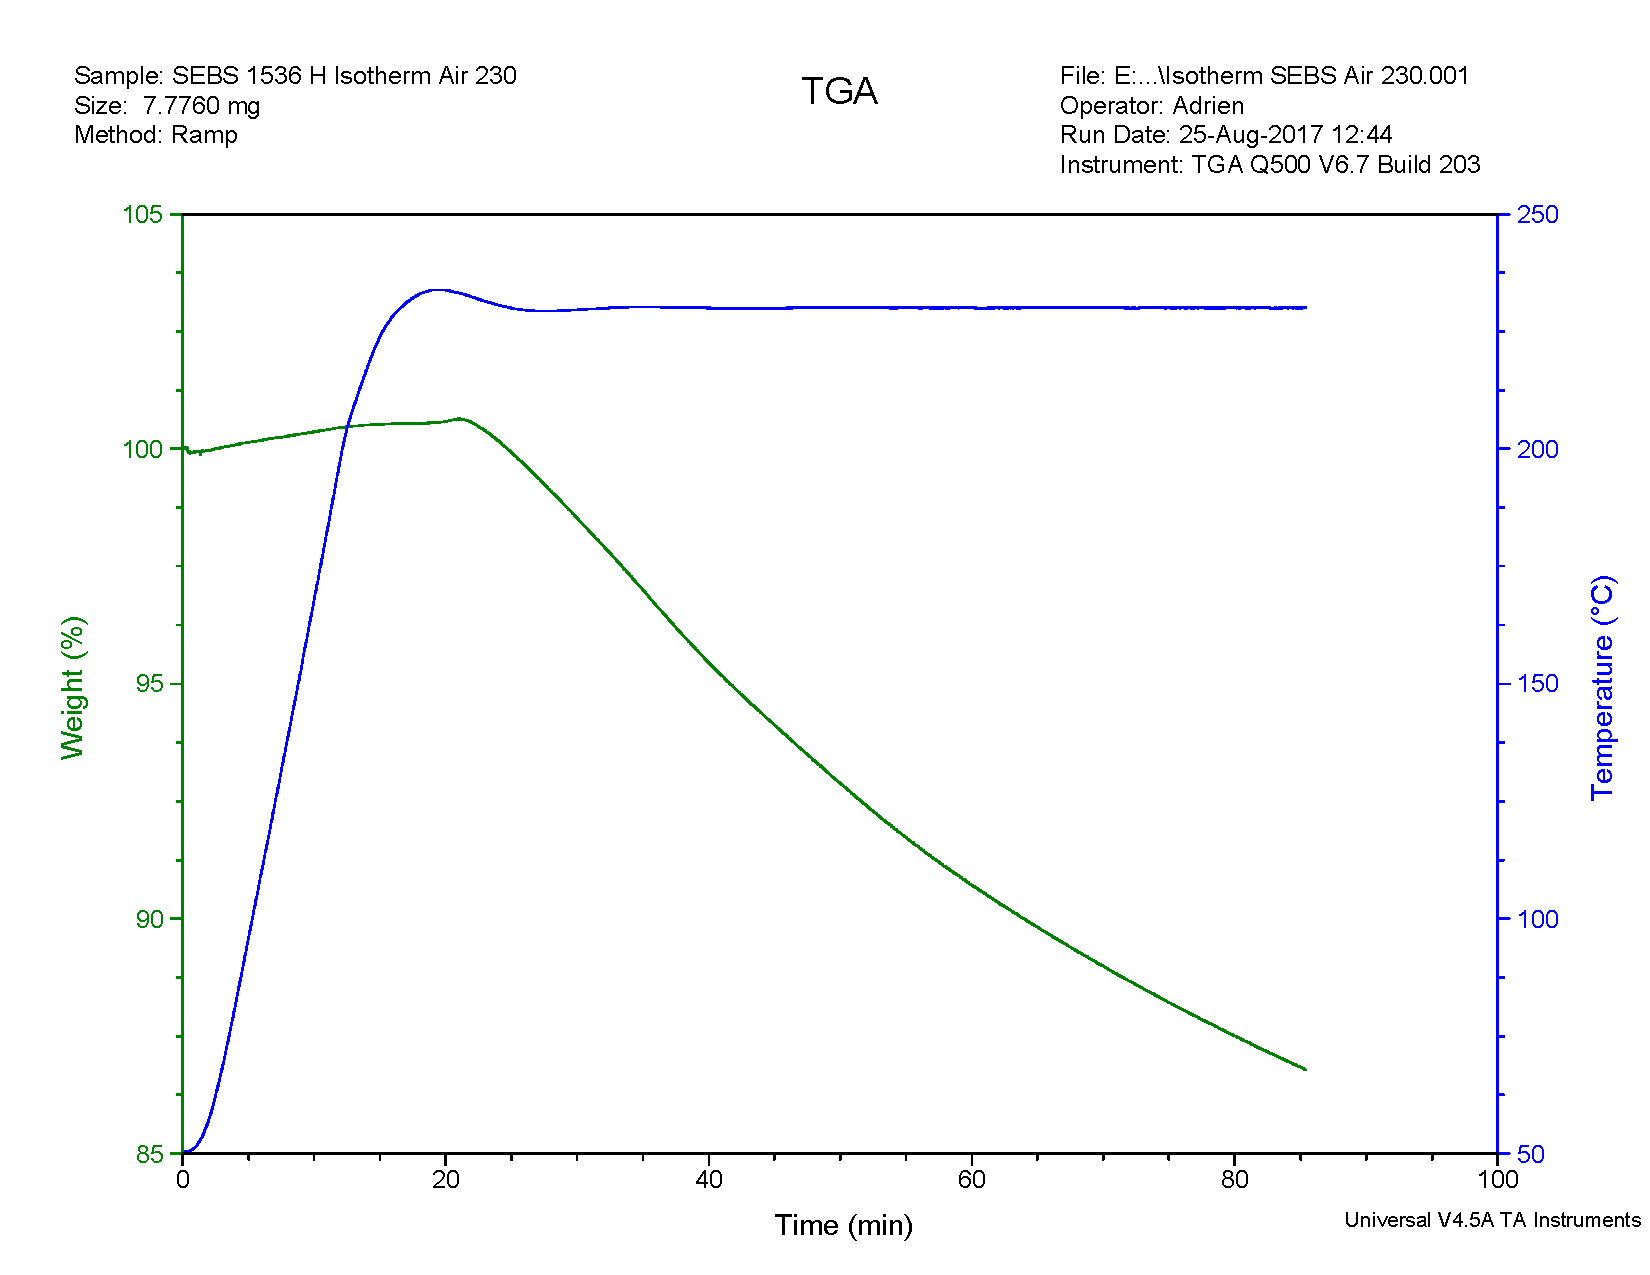
\includegraphics[width=0.75\textwidth]{TGA_SEBS_1536H_Air_Isotherm_230.pdf}
	}
	\caption{Résultats en TGA isotherme pour l'élastomère SEBS dans l'air à a) \SI{200}{\celsius} at b) \SI{230}{\celsius}}
	\label{fig:TGA_iso_SEBS_air}
\end{figure}

\begin{figure}[h]
	\centering
	\subfigure[]
	{\label{fig:TGA_iso_SEBS_N2_275} 								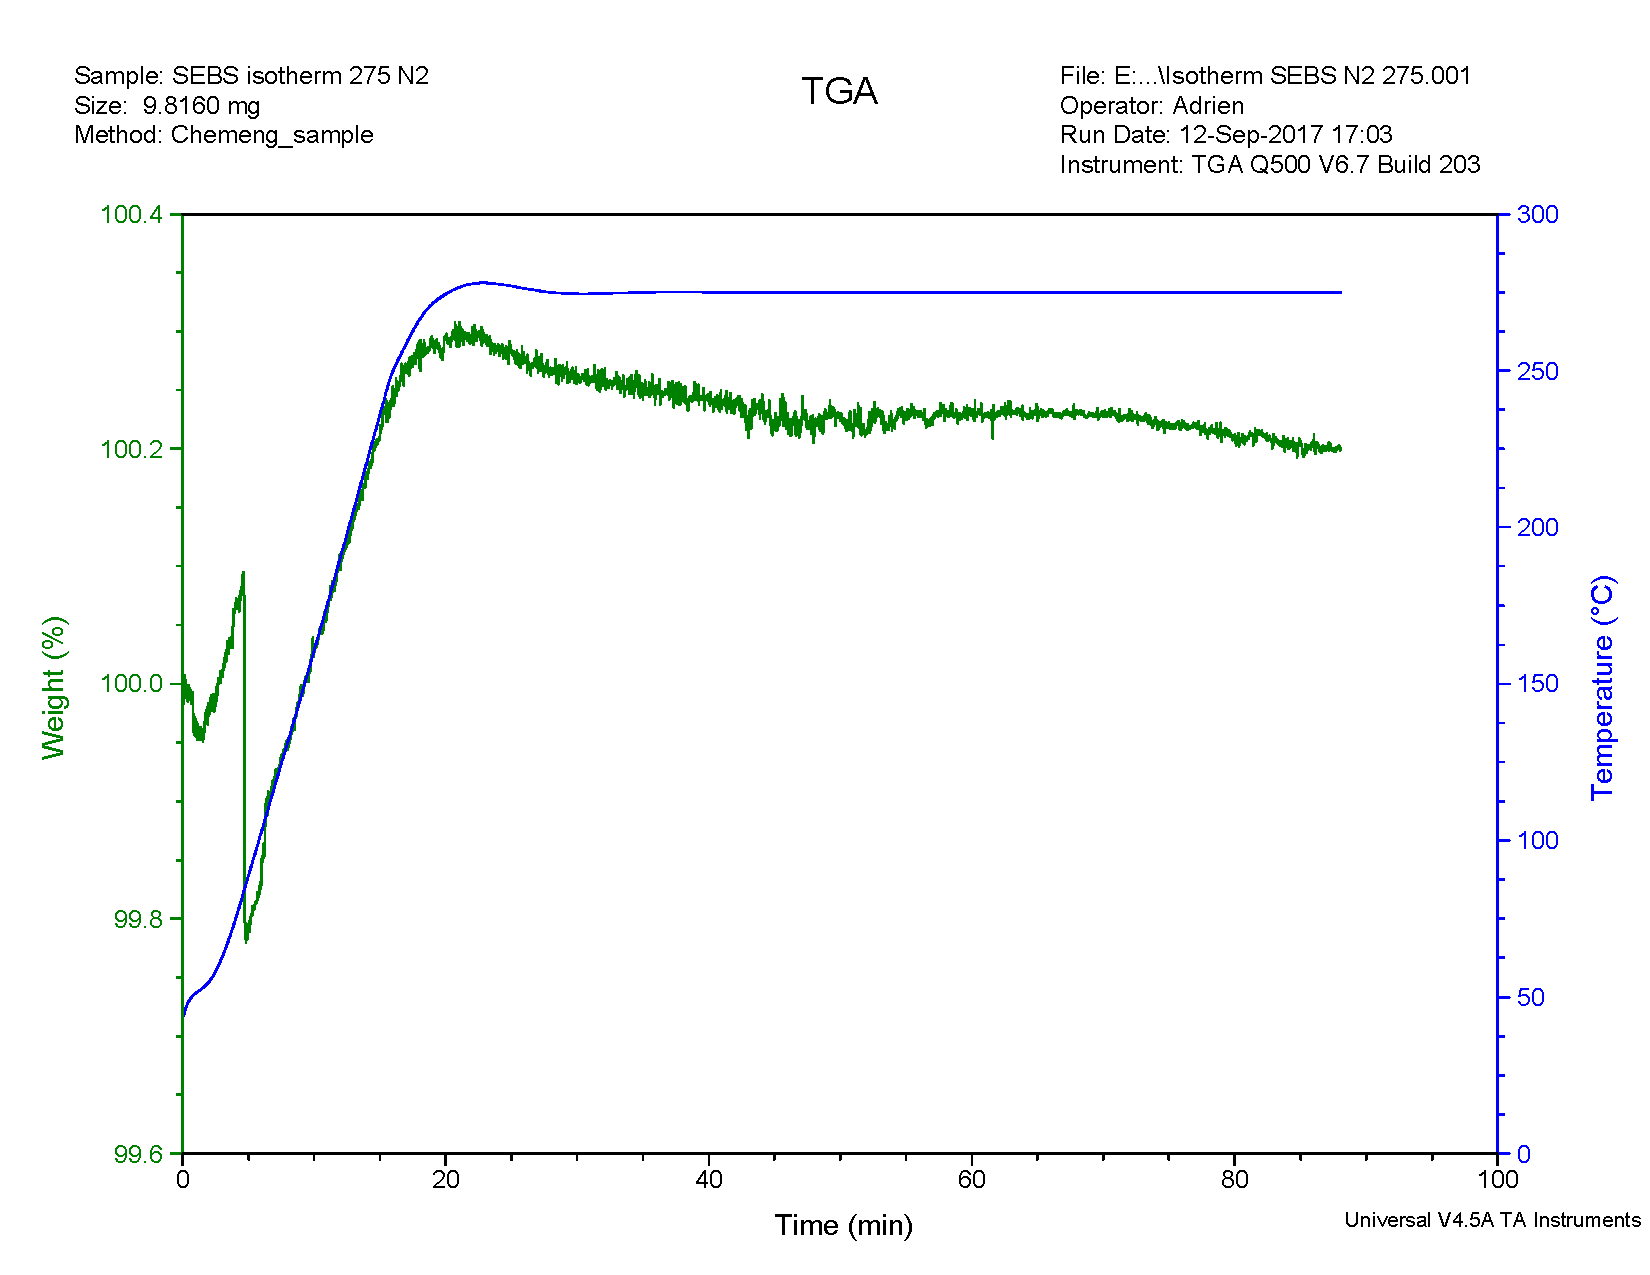
\includegraphics[width=0.75\textwidth]{TGA_SEBS_1536H_N2_Isotherm_275.pdf}
	}\\
	\subfigure[]
	{\label{fig:TGA_iso_SEBS_N2_290}
		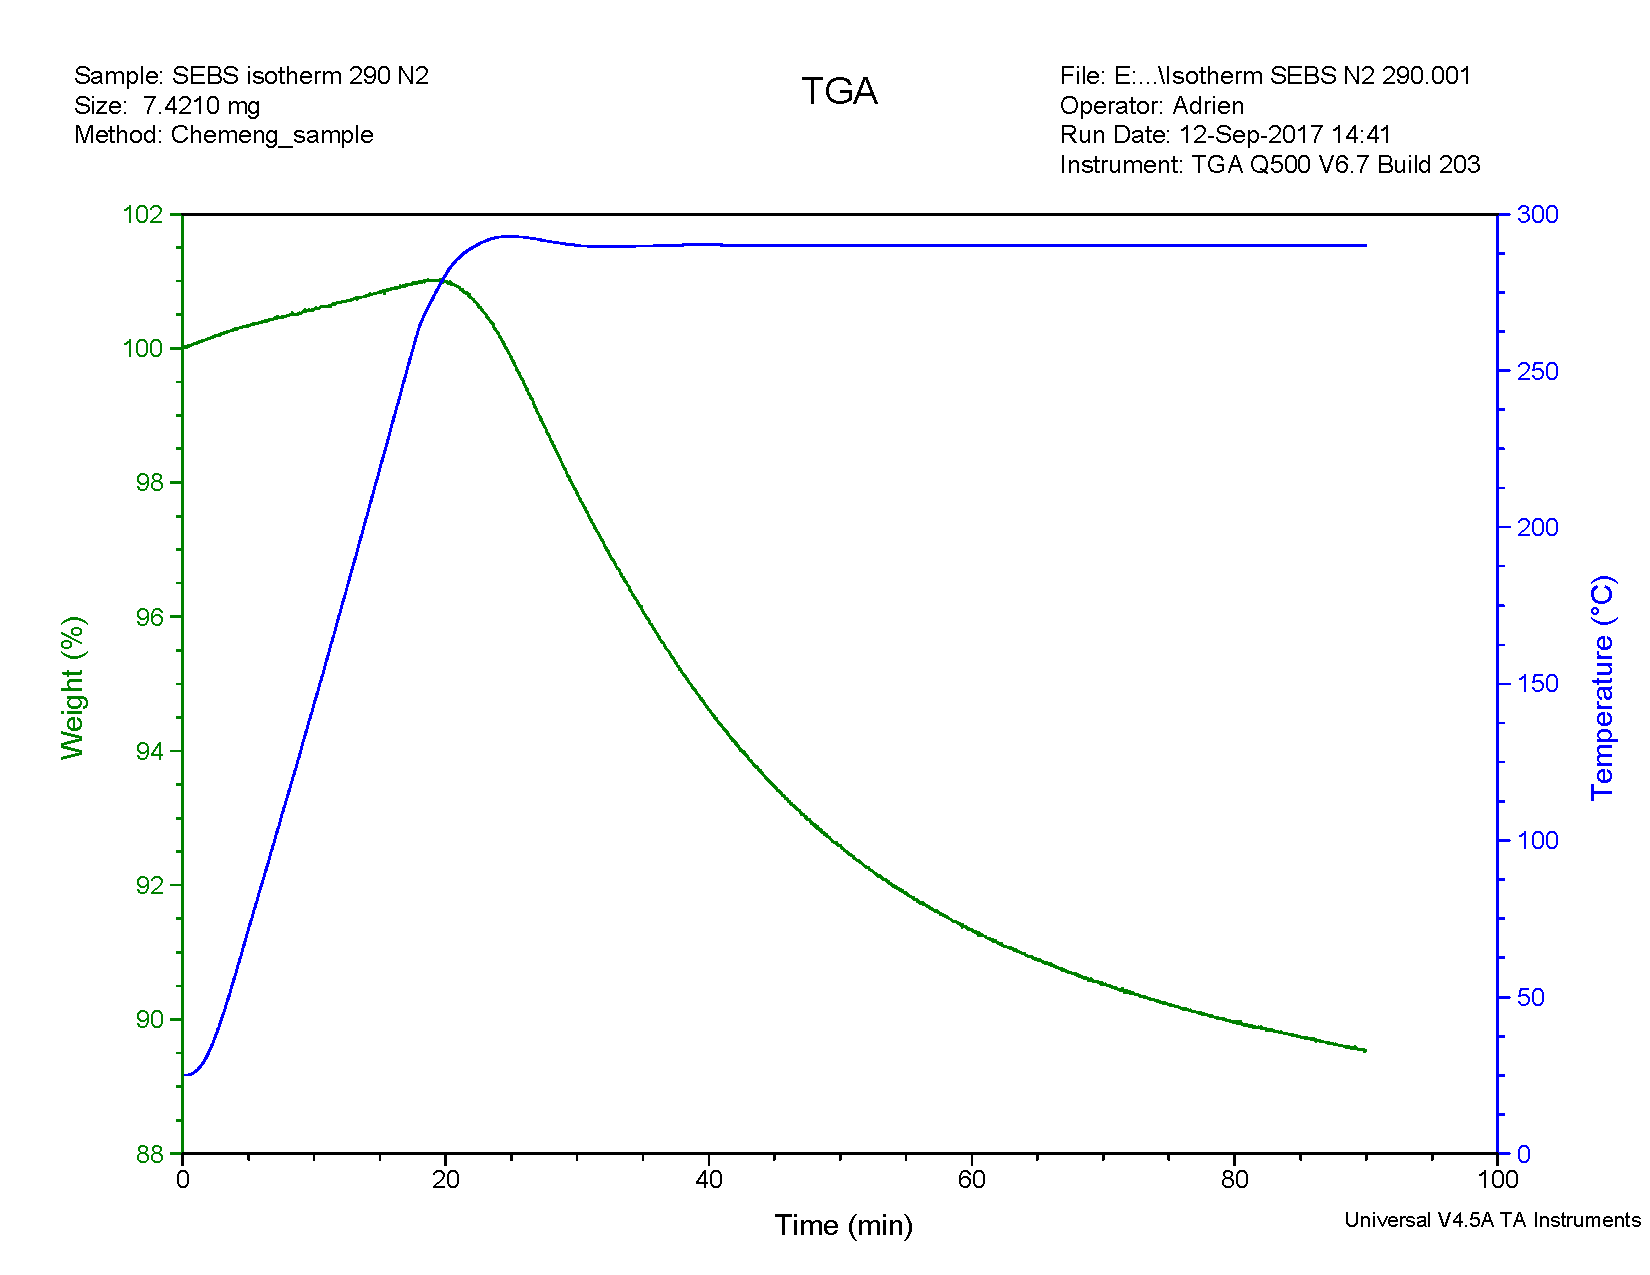
\includegraphics[width=0.75\textwidth]{TGA_SEBS_1536H_N2_Isotherm_290.pdf}
	}
	\caption{Résultats en TGA isotherme pour l'élastomère SEBS sous une atmosphère d'azote à a) \SI{275}{\celsius} at b) \SI{290}{\celsius}}
	\label{fig:TGA_iso_SEBS_N2}
\end{figure}

\section{Essais de soudage isotherme}

La stabilité thermique de l'élastomère SEBS a été jugée suffisamment bonne pour tenter de réaliser des jonctions soudées. 
Les premiers essais de soudage ont été réalisés dans une étuve sous vide en isotherme afin d'éviter de dégrader l'élastomère et de donner aux chaînes de polymère une longue période de temps afin qu'elles aient le temps de migrer au travers de l'interface. 
Lors du premier test, l'échantillon (Fig. \ref{fig:weldstack_SEBS}) dans l'étuve a été chauffé jusqu'à une température de \SI[locale=FR]{260}{\celsius}, pendant 24 heures. 
Les résultats obtenus démontrent le manque de tenue en température de l'élastomère et qu'un temps de soudage trop élevé lui permet de fluer en dehors de la zone à souder (Fig. \ref{fig:etuve_SEBS_flat}). 
De plus, dans la zone où de l'élastomère était encore en contact avec le nanocomposite, il était facile de le peler (Fig. \ref{fig:etuve_SEBS_pelage}). 
Ce test n'a pas été jugé totalement concluant puisqu'en raison du fluage de l'élastomère, la pression sur ce dernier n'était pas uniforme durant le test. 
La faible pression pourrait avoir nui au processus de diffusion des chaînes. 

\begin{figure}[h!]
	\centering
	\subfigure[]
	{\label{fig:weldstack_SEBS} 								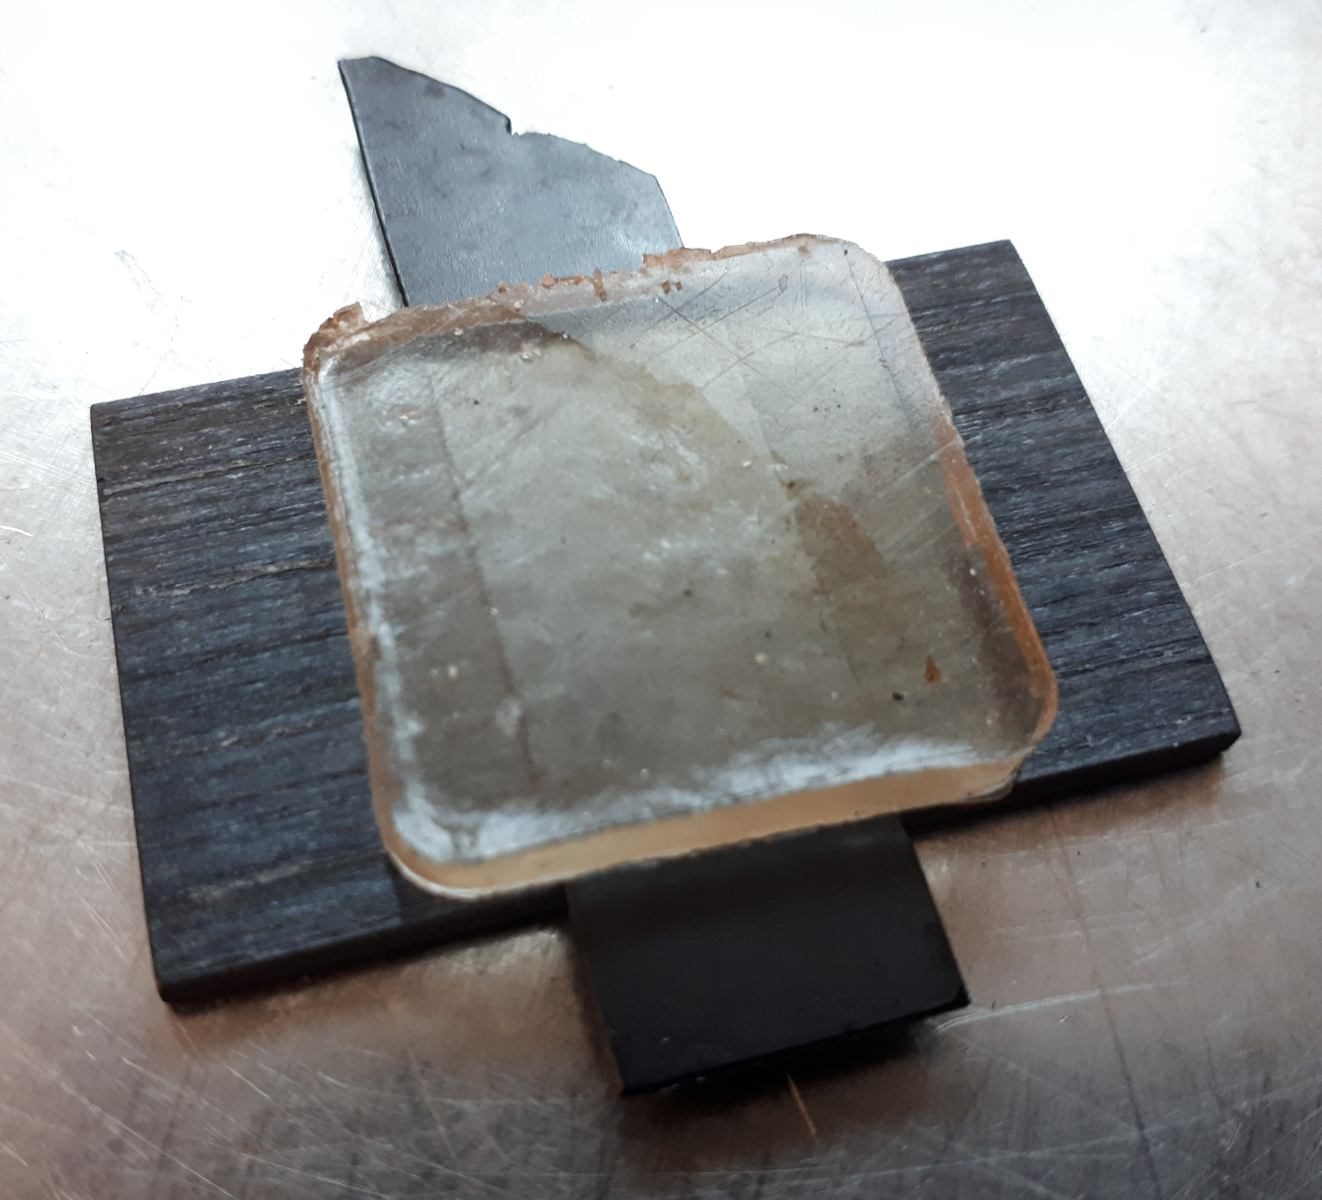
\includegraphics[height=4.2cm]{20171215_091800_crop_resize.jpg}
	} \
	\subfigure[]
	{\label{fig:etuve_SEBS_flat} 								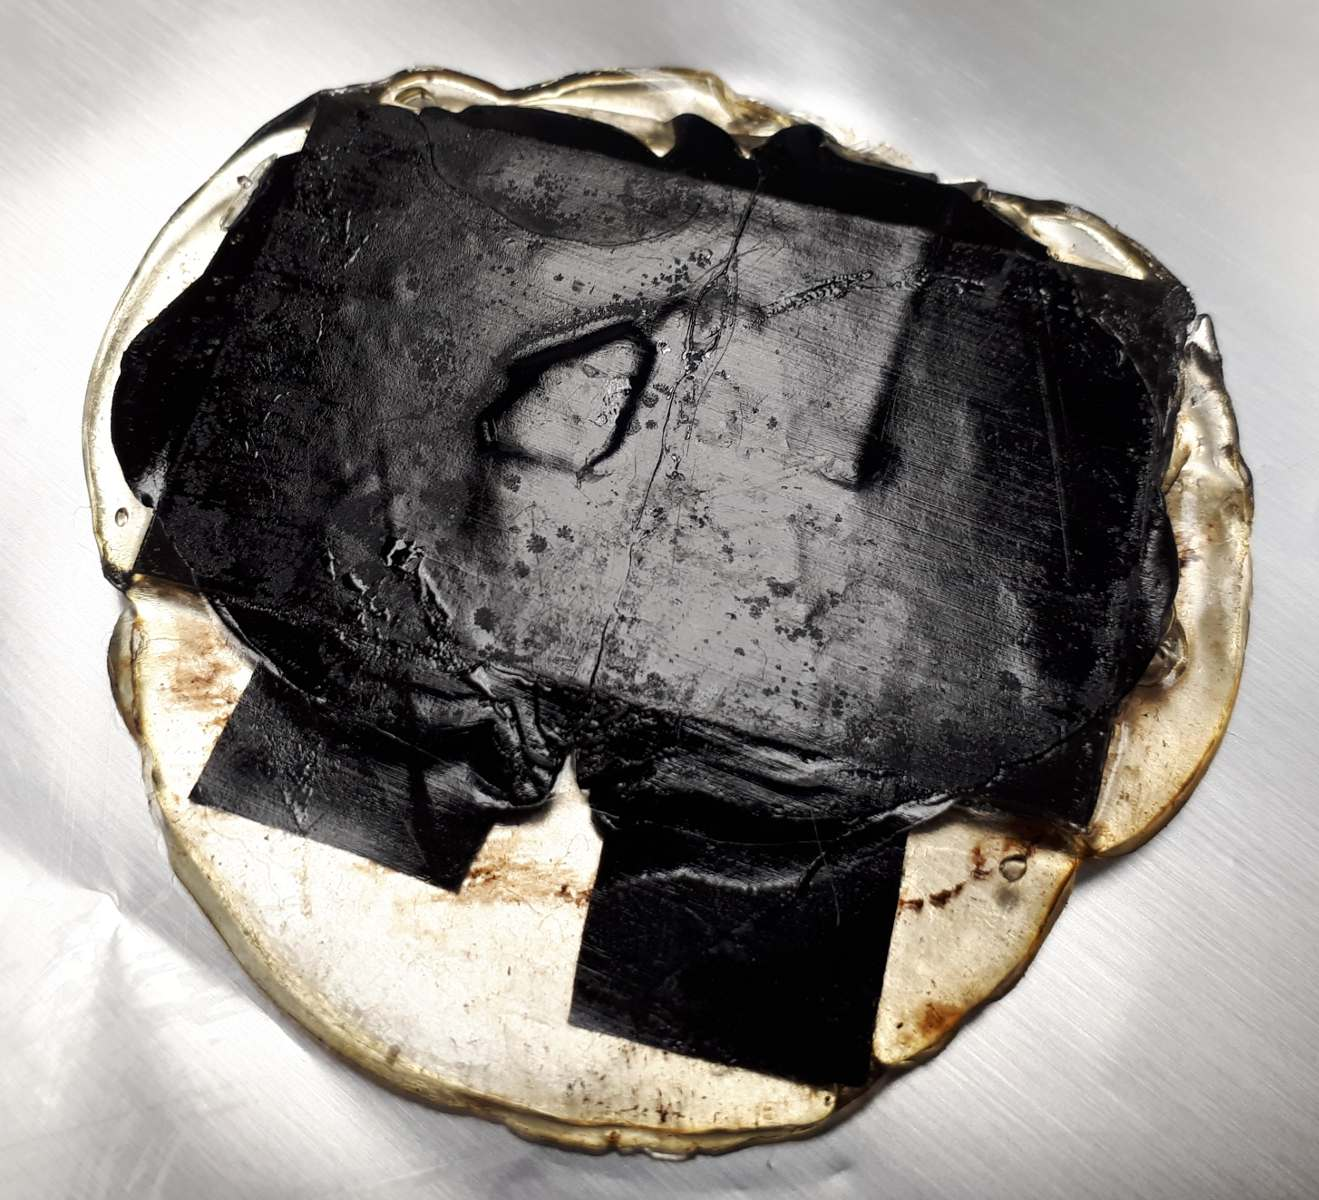
\includegraphics[height=4.2cm]{20180117_153151_crop_resize.jpg}
	} \
	\subfigure[]
	{\label{fig:etuve_SEBS_pelage}
		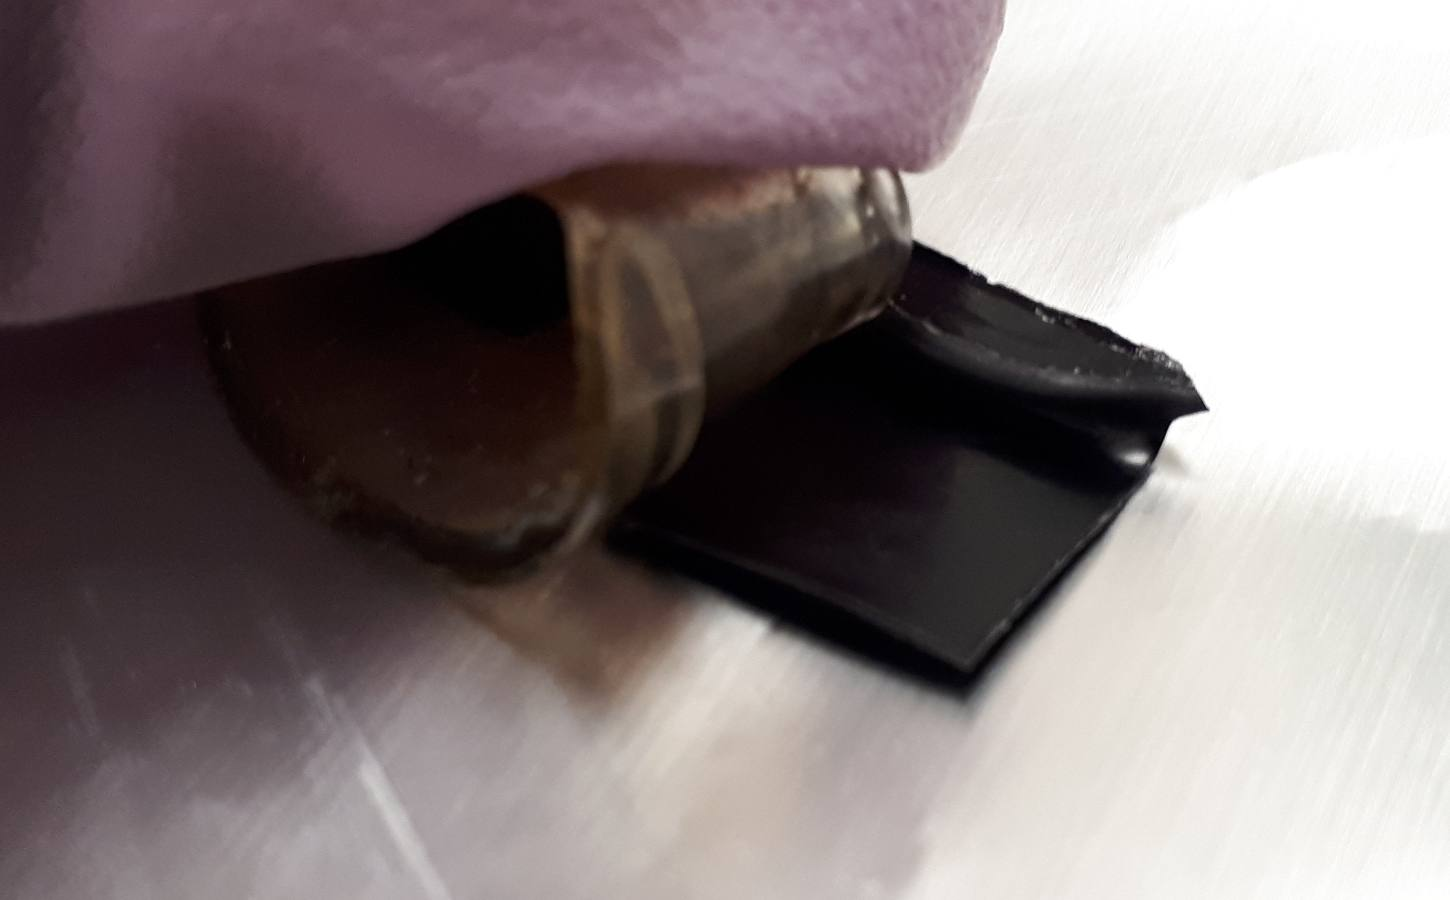
\includegraphics[height=3.5cm]{20180117_154300_crop_resize.jpg}
	}
	\caption{Essai de soudage dans une étuve sous vide à \SI{260}{\celsius} pour l'élastomère SEBS présentant a) la préparation de l'échantillon, b) l'échantillon à la sortie de l'étuve et c) le pelage de l'élastomère}
	\label{fig:etuve_SEBS}
\end{figure}

\begin{figure}[h]
	\centering
	\subfigure[]
	{\label{fig:welds_SEBS_presse} 								
		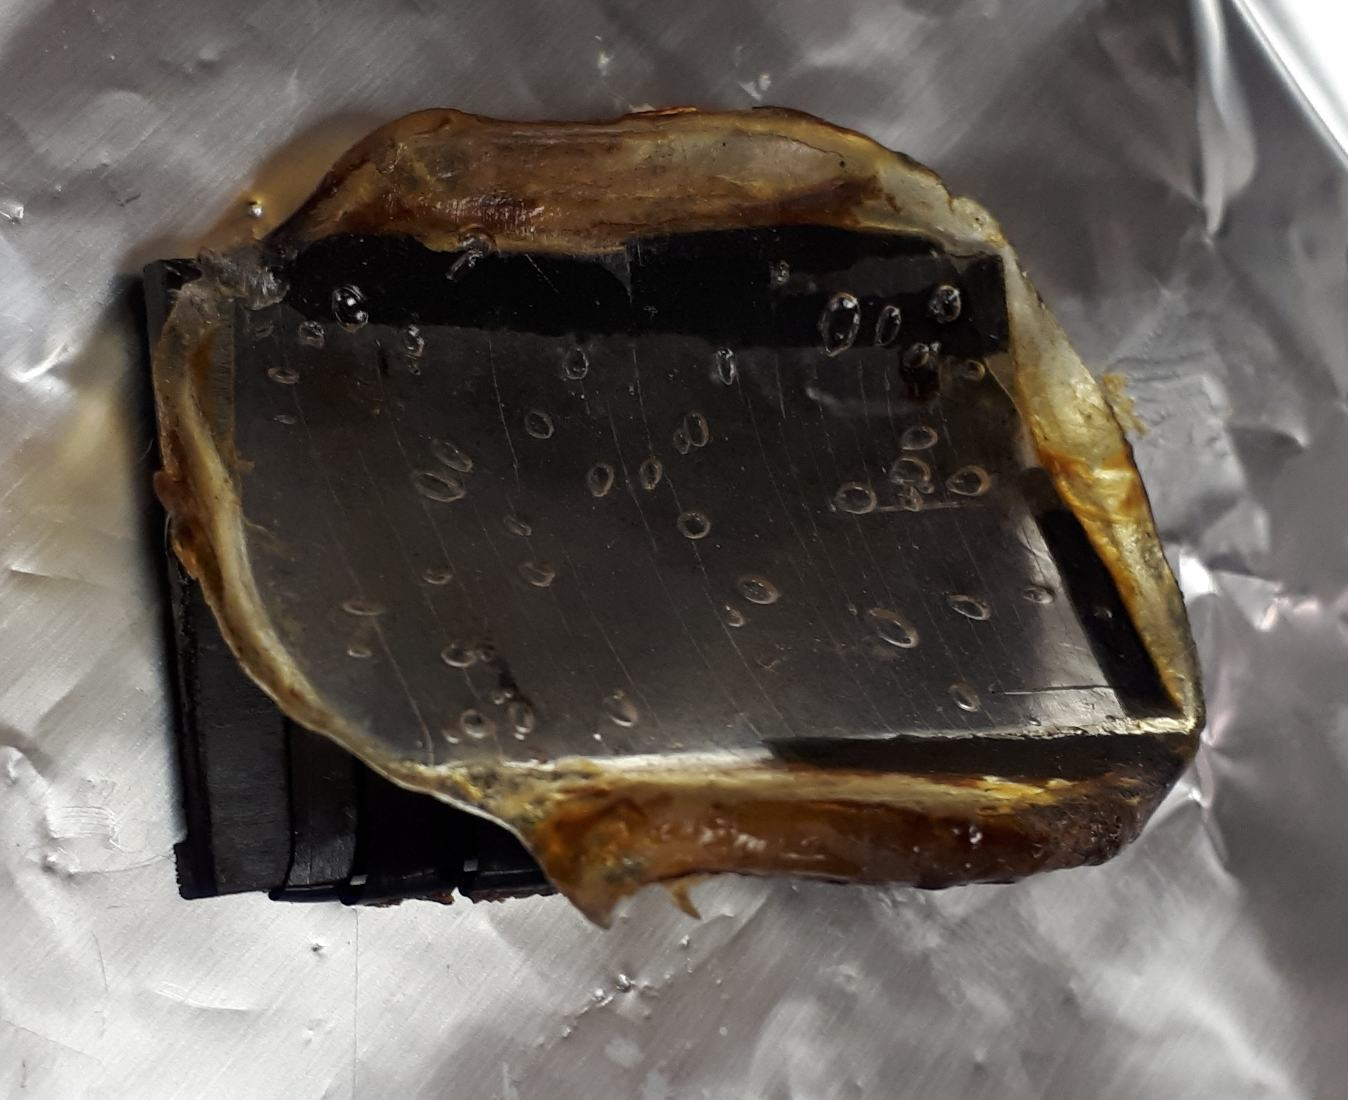
\includegraphics[height=6.cm]{20180124_142710_crop_resize.jpg}
	} \qquad
	\subfigure[]
	{\label{fig:welds_SEBS_presse_pelage} 								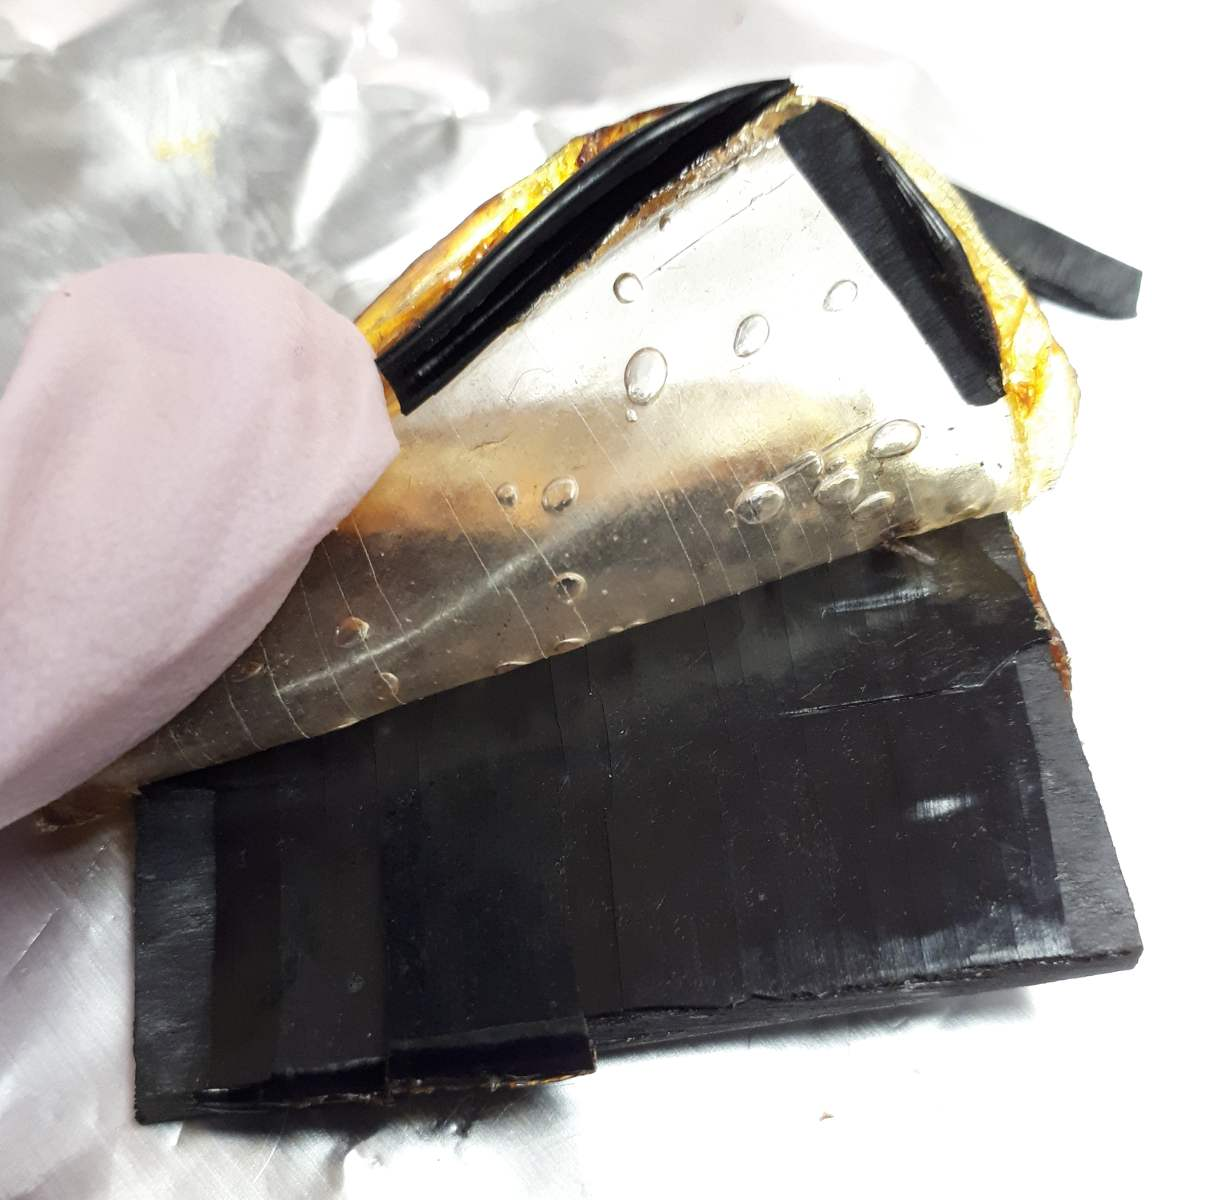
\includegraphics[height=6.cm]{20180124_142724_crop_resize.jpg}
	}
	\caption{Essai de soudage à la presse à \SI{260}{\celsius} pour l'élastomère SEBS présentant a) l'échantillon à la sortir de la presse et b) le pelage de l'élastomère}
	\label{fig:presse_SEBS}
\end{figure}

\FloatBarrier
Suite aux premiers résultats à l'étuve, il a été décidé de réaliser un essai de soudage à la presse chauffante avec l'élastomère SEBS. 
Cet essai avait pour but de tenter un temps de soudage plus court, mais avec une pression de contact plus élevée. 
Cependant, la force minimale que la presse a pu appliquer durant ce test a causé une pression de \SI[locale=FR]{5}{\mega\pascal} qui a entrainé le fluage de l'élastomère (Fig. \ref{fig:welds_SEBS_presse}). 
Encore une fois, l'élastomère a pu être facilement séparé du nanocomposite (Fig. \ref{fig:welds_SEBS_presse_pelage}). 
En raison de l'ensemble des résultats obtenus pour le SEBS, les essais pour cette famille de polymère se sont conclus à ce point. 